\apendice{Documentación técnica de programación}

\section{Introducción}

En esta sección se describirá la documentación técnica de programación del proyecto. Se incluye la estructura de directorios utilizada, la instalación y ejecución del proyecto, así como las pruebas realizadas.

\section{Estructura de directorios}
\begin{itemize}
\item \textbf{/}: Directorio raíz. Contiene los ficheros de configuración de la instalación mediante \emph{setuptools}, un script de instalación rápida y el fichero README con información sobre el proyecto.
\item \textbf{/backend/}: Contiene los diferentes paquetes con el código fuente de la aplicación que será ejecutada en el sistema de control del \emph{drone}.
\item \textbf{/docs/}: Contiene la documentación del proyecto.
\item \textbf{/frontend/}: Contiene los diferentes paquetes con el código fuente de la aplicación que será ejecutada en el servidor web.
\item \textbf{/test/}: Contiene algunos test generados para comprobar el funcionamiento de las clases, así como la implementación del algoritmo de campos potenciales, que podría establecerse como \emph{deprecated} en favor del VFH.
\end{itemize}


\section{Manual del programador}
Para trabajar con el proyecto es necesario tener instalado el siguiente software:

\begin{itemize}
\item JetBrains PyCharm IDE.
\item Git.
\item Un cliente de escritorio para Git (recomendable pero no indispensable), como GitKraken.
\item Una shell capaz de ejecutar un script bash. Windows dispone de CygWin, para sistemas operativos con base Unix esta está disponible por defecto. 
\item Python 3.5+.
\end{itemize}

El resto de dependencias, referenciadas a continuación, serán instaladas mediante el script de instalación:
\begin{itemize}
\item \textbf{BackEnd}:
\begin{itemize}
	\item Numpy
	\item SciPy
	\item PySerial
	\item Bluetin\_Echo
\end{itemize}
\item \textbf{FrontEnd}:
\begin{itemize}
	\item Flask-Login
	\item Flask-WTF
	\item Flask-SQLAlchemy
	\item Flask-Migrate
	\item Flask-SocketIO
	\item Eventlet
	\item Flask
\end{itemize}
\end{itemize}


Además, si se desea llevar a cabo pruebas reales del sistema, es necesario disponer del siguiente hardware: 

\begin{itemize}
\item Raspberry Pi 3B o similar con sistema operativo Raspbian Stretch.
\item Una cámara compatible con RaspberryPi. En este desarrollo se ha hecho uso de una PiNoIR, por no tener filtro de infrarrojos, de manera que se puede usar en momentos de baja luminosidad.
\item Una controladora de vuelo compatible con \textit{BetaFlight}\footnote{Firmware que se ejecutará en la controladora de vuelo. Dispone de una aplicación para configurar la misma.} o similar. 
\item 6x Sensores de distancia por ultrasonidos \textit{HC-SR04}.
\item Regulador de voltaje para no exceder el voltaje máximo de entrada en la RaspberryPi. 
\item LEDs infrarrojos.
\item Un \emph{drone} sobre el que montar los dispositivos.
\item Una emisora compatible con el sistema operativo, y reconocible por este como un joysitck. En este desarrollo se ha empleado una emisora \textit{FrSky Taranis X9D Plus}.
\end{itemize}

A continuación se detalla como instalar y configurar los requerimientos arriba descritos: 

\subsection{RaspberryPi y Raspbian}
\label{subsec:raspbian}
Este apartado se encuentra en primer lugar, dadas las múltiples referencias al acceso a la RaspberryPi que se darán a continuación. 

Para conseguir la última imagen de instalación de Raspbian se puede acceder a \citep{wiki:raspbian}. En este proyecto se ha utilizado la imagen \emph{lite} del sistema, que no dispone de interfaz de usuario, y es más ligera. (Extraido del documento de memoria, apartado 3):

Una vez descargado el sistema, este ha sido instalado en una micro SD mediante el siguiente procedimiento por consola\footnote{Realizado en OSX, aunque en Linux es muy similar}:
\begin{itemize}
\item\code{diskutil list} Permite localizar el dispositivo en el que se encuentra la tarjeta. En nuestro caso \code{/dev/disk4}
\item\code{diskutil umountDisk /dev/disk4} Permite desmontar el volumen. 
\item\code{sudo dd if=raspbian-stretch.img of=/dev/rdisk4 bs=1m} El comando \code{dd} copia la entrada estándar a la salida estándar. Mediante \code{if/of} se establece el fichero de entrada/salida. Mediante \code{bs} se establece el tamaño de bloque a copiar. Se está utilizando \code{/dev/\underline{\textbf{r}}disk4} en lugar de \code{/dev/disk4} debido a la capacidad de OSX de trabajar con dispositivos en bruto, \textit{raw}, de forma que es posible acceder al dispositivo de forma directa\footnote{Véase \code{man hdiutil}, sección \textit{DEVICE SPECIAL FILES}}, sin almacenar en un buffer la lectura del archivo, proporcionando velocidades de escritura/lectura hasta 20 veces más rápidas.
\end{itemize}

\subsection{JetBrains PyCharm IDE}
\label{subsec:pycharm}
El IDE desarrollado por JetBrains es posiblemente el más avanzado para la creación de aplicaciones en Python. Se puede descargar desde \citep{wiki:PyCharm}, escogiendo el sistema operativo, y su instalación se basa en seguir el asistente de instalación.

Sin embargo, si se va a trabajar con una RaspberryPi, es conveniente configurar esta como destino del despliegue del \emph{backend}, de manera que se pueda realizar el \emph{debuggeo} de las aplicaciones de forma remota, así como su despliegue. 

Accediendo a las preferencias del IDE, en el apartado \emph{Build, Execution, Deployment} y bajo el subapartado \emph{Deployment}, se puede establecer la configuración del dispositivo sobre el que realizar el despliegue, tal y como se muestra en la figura \ref{fig:pycharmDeployConfig}.


\begin{figure}[H]
	\centering
	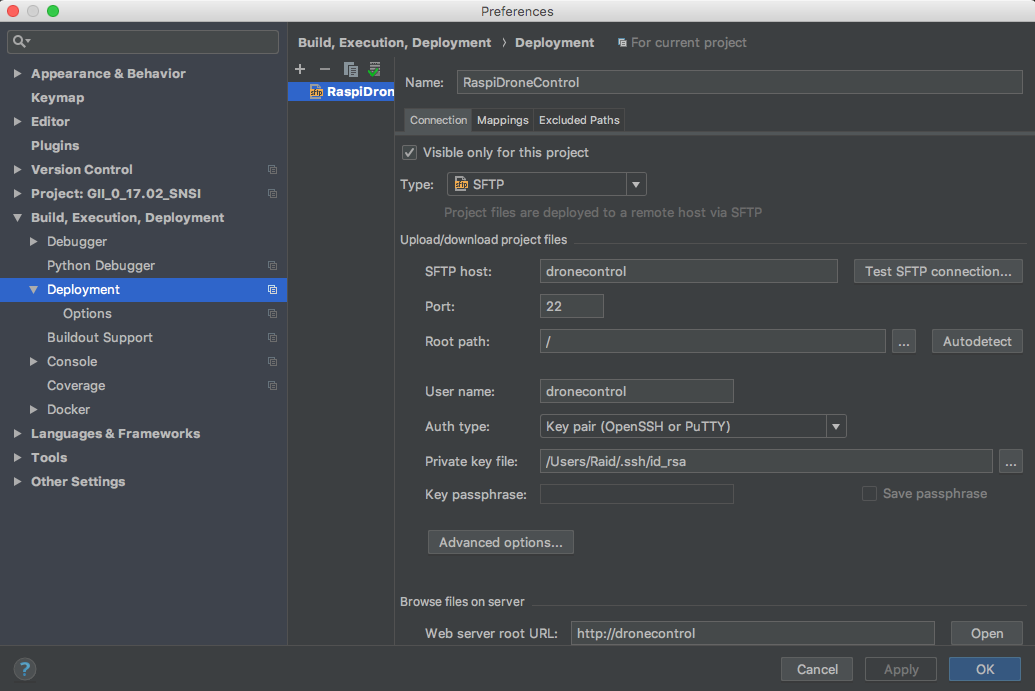
\includegraphics[width=1\textwidth]{pycharmDeployConfig}
	\caption[PyCharm. Configuración de despliegue]{Configuración del despliegue remoto en PyCharm.}\label{fig:pycharmDeployConfig}
\end{figure}

Conviene configurar el acceso a la RaspberryPi mediante claves públicas. Para el detalle de como configurar el acceso, y generar las claves públicas ver la subsección \ref{subsub:sshconfig}.

Se debe configurar también el intérprete remoto para la ejecución y \emph{debug} de aplicaciones. Puede hacerse en PyCharm accediendo a las preferencias del IDE, en el apartado \emph{Project: GII\_0\_17.02\_SNSI} y bajo el subapartado \emph{Project Interpreter}, se puede establecer la configuración del dispositivo sobre el que realizar el despliegue, tal y como se muestra en la figura \ref{fig:pycharmRemoteDebug}.

\begin{figure}[H]
	\centering
	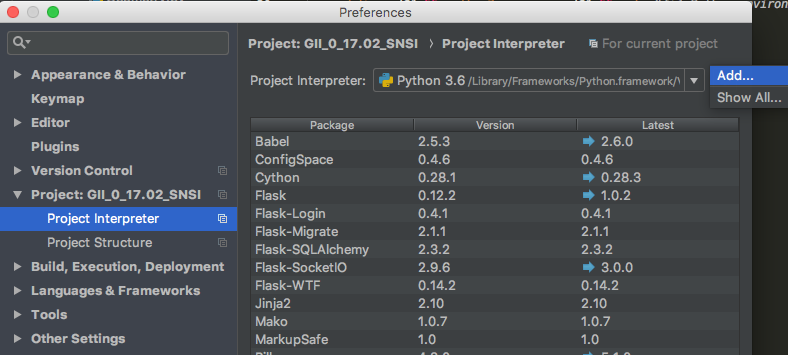
\includegraphics[width=1\textwidth]{pycharmRemoteDebug}
	\caption[PyCharm. Configuración de intérprete remoto]{Configuración del intérprete remoto en PyCharm.}\label{fig:pycharmRemoteDebug}
\end{figure}

Se especificaría el host al que conectarse via SSH, tal y como se muestra en la imagen \ref{fig:sshinterpreter}.

\begin{figure}[H]
	\centering
	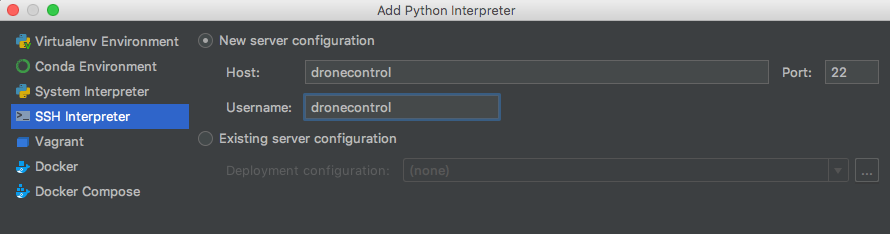
\includegraphics[width=1\textwidth]{sshinterpreter}
	\caption[PyCharm. Configuración de intérprete remoto. SSH]{Configuración del intérprete remoto en PyCharm vía SSH.}\label{fig:sshinterpreter}
\end{figure}

Y por último se selecciona el intérprete existente en el entorno virtual generado mediante el script de instalación, ver subsección \ref{subsec:installersh}, y la correspondencia de carpetas, como se muestra en la imagen \ref{fig:sshvenv}.
\begin{figure}[H]
	\centering
	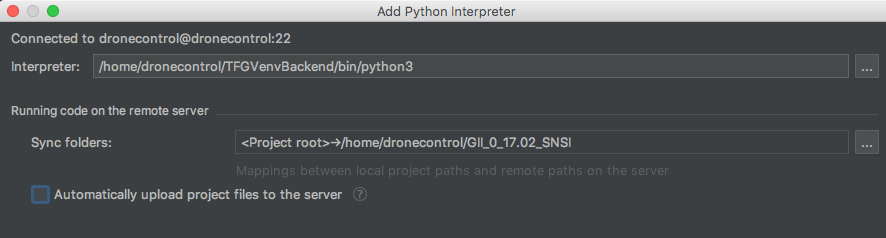
\includegraphics[width=1\textwidth]{sshvenv}
	\caption[PyCharm. Configuración de intérprete remoto. VirtualEnv]{Configuración del intérprete remoto en PyCharm vía SSH en un \emph{Virtual Environment}.}\label{fig:sshvenv}
\end{figure}



\subsubsection{Configuración SSH}
\label{subsub:sshconfig}

Como añadido al anexo, aunque se encuentra disponible en la sección 3 de la memoria, se generan las claves públicas a usar en PyCharm para acceder a la RaspberryPi de forma remota, siguiendo los siguientes pasos:

\begin{itemize}
\item Generar el par de claves pública-privada en el cliente mediante el comando \code{ssh-keygen}
\item Copiar la clave pública del cliente en el archivo \code{.ssh/authorized\_keys} de la carpeta \code{home} del usuario a utilizar en el sistema remoto.
\item Editar el archivo \code{/etc/ssh/sshd\_config} para:
	\begin{itemize}
	\item permitir unicamente acceso a usuarios que envíen una clave pública contenida en \code{authorized\_keys}.
	\item desactivar el acceso al usuario root, estableciendo la propiedad \code{PermitRootLogin} a \code{no}.
	\item desactivar el acceso por contraseña, estsableciendo la propiedad \code{PasswordAuthentication} a \code{no}.
	\end{itemize}	 
\end{itemize} 


\subsection{Installación de Git}
Para hacer uso de las capacidades de un sistema de control de versiones, se utilizará Git. Se puede obtener desde \citep{wiki:getGit}. Aunque para comodidad, se hará uso de un entorno de escritorio, ver subsección \ref{subsec:gitkraken}.

\subsection{Installación de GitKraken}
\label{subsec:gitkraken}
GitKraken es un entorno de escritorio para Git. Tiene integración con GitHub y permite hacer una gran cantidad de tareas de forma muy cómoda. Puede obtenerse a través de \citep{wiki:GitKraken}, y su instalación se basa en seguir el asistente, así como la configuración de acceso al repositorio local, y remoto.



\subsection{Conexión de Hardware}

Si se desea probar el proyecto, y desplegarlo en una RaspberryPi con acceso a todos los sensores, se deberían considerar los siguientes pasos: 

\begin{itemize}
\item Arrancar la RaspberryPi con la imagen grabada, tal y como se explicó en la subsección \ref{subsec:raspbian} y \textbf{SIN} conectar los sensores\footnote{Es muy importante no conectar los sensores hasta estar 100\% seguros de que no existe ningún pin del componente GPIO de la RaspberryPi enviando un voltaje a un periférico conectado a él. Esto podría causar daños en los sensores si el voltaje es aplicado al pin de salida en lugar de al pin de entrada.}
\item Una vez arrancado el sistema, se puede acceder a él vía SSH. Se deberá dar acceso al usuario al puerto serie ya que, por defecto, no lo tiene. Para ello se debe añadir al usuario al grupo \code{dialout}.
\item Se puede <<limpiar>> el estado de los pines mediante un simple script de Python, importando \emph{RPi.GPIO} y llamando al método \emph{cleanup}.
\item Para conectar la RaspberryPi a la controladora de vuelo se puede usar un puerto USB, y un cable con un extremo USB-A y el otro \emph{microUSB}.
\item El diagrama de conexionado de los sensores de ultrasonidos puede verse en la figura \ref{fig:concepHCPi}. 
\begin{figure}[H]
	\centering
	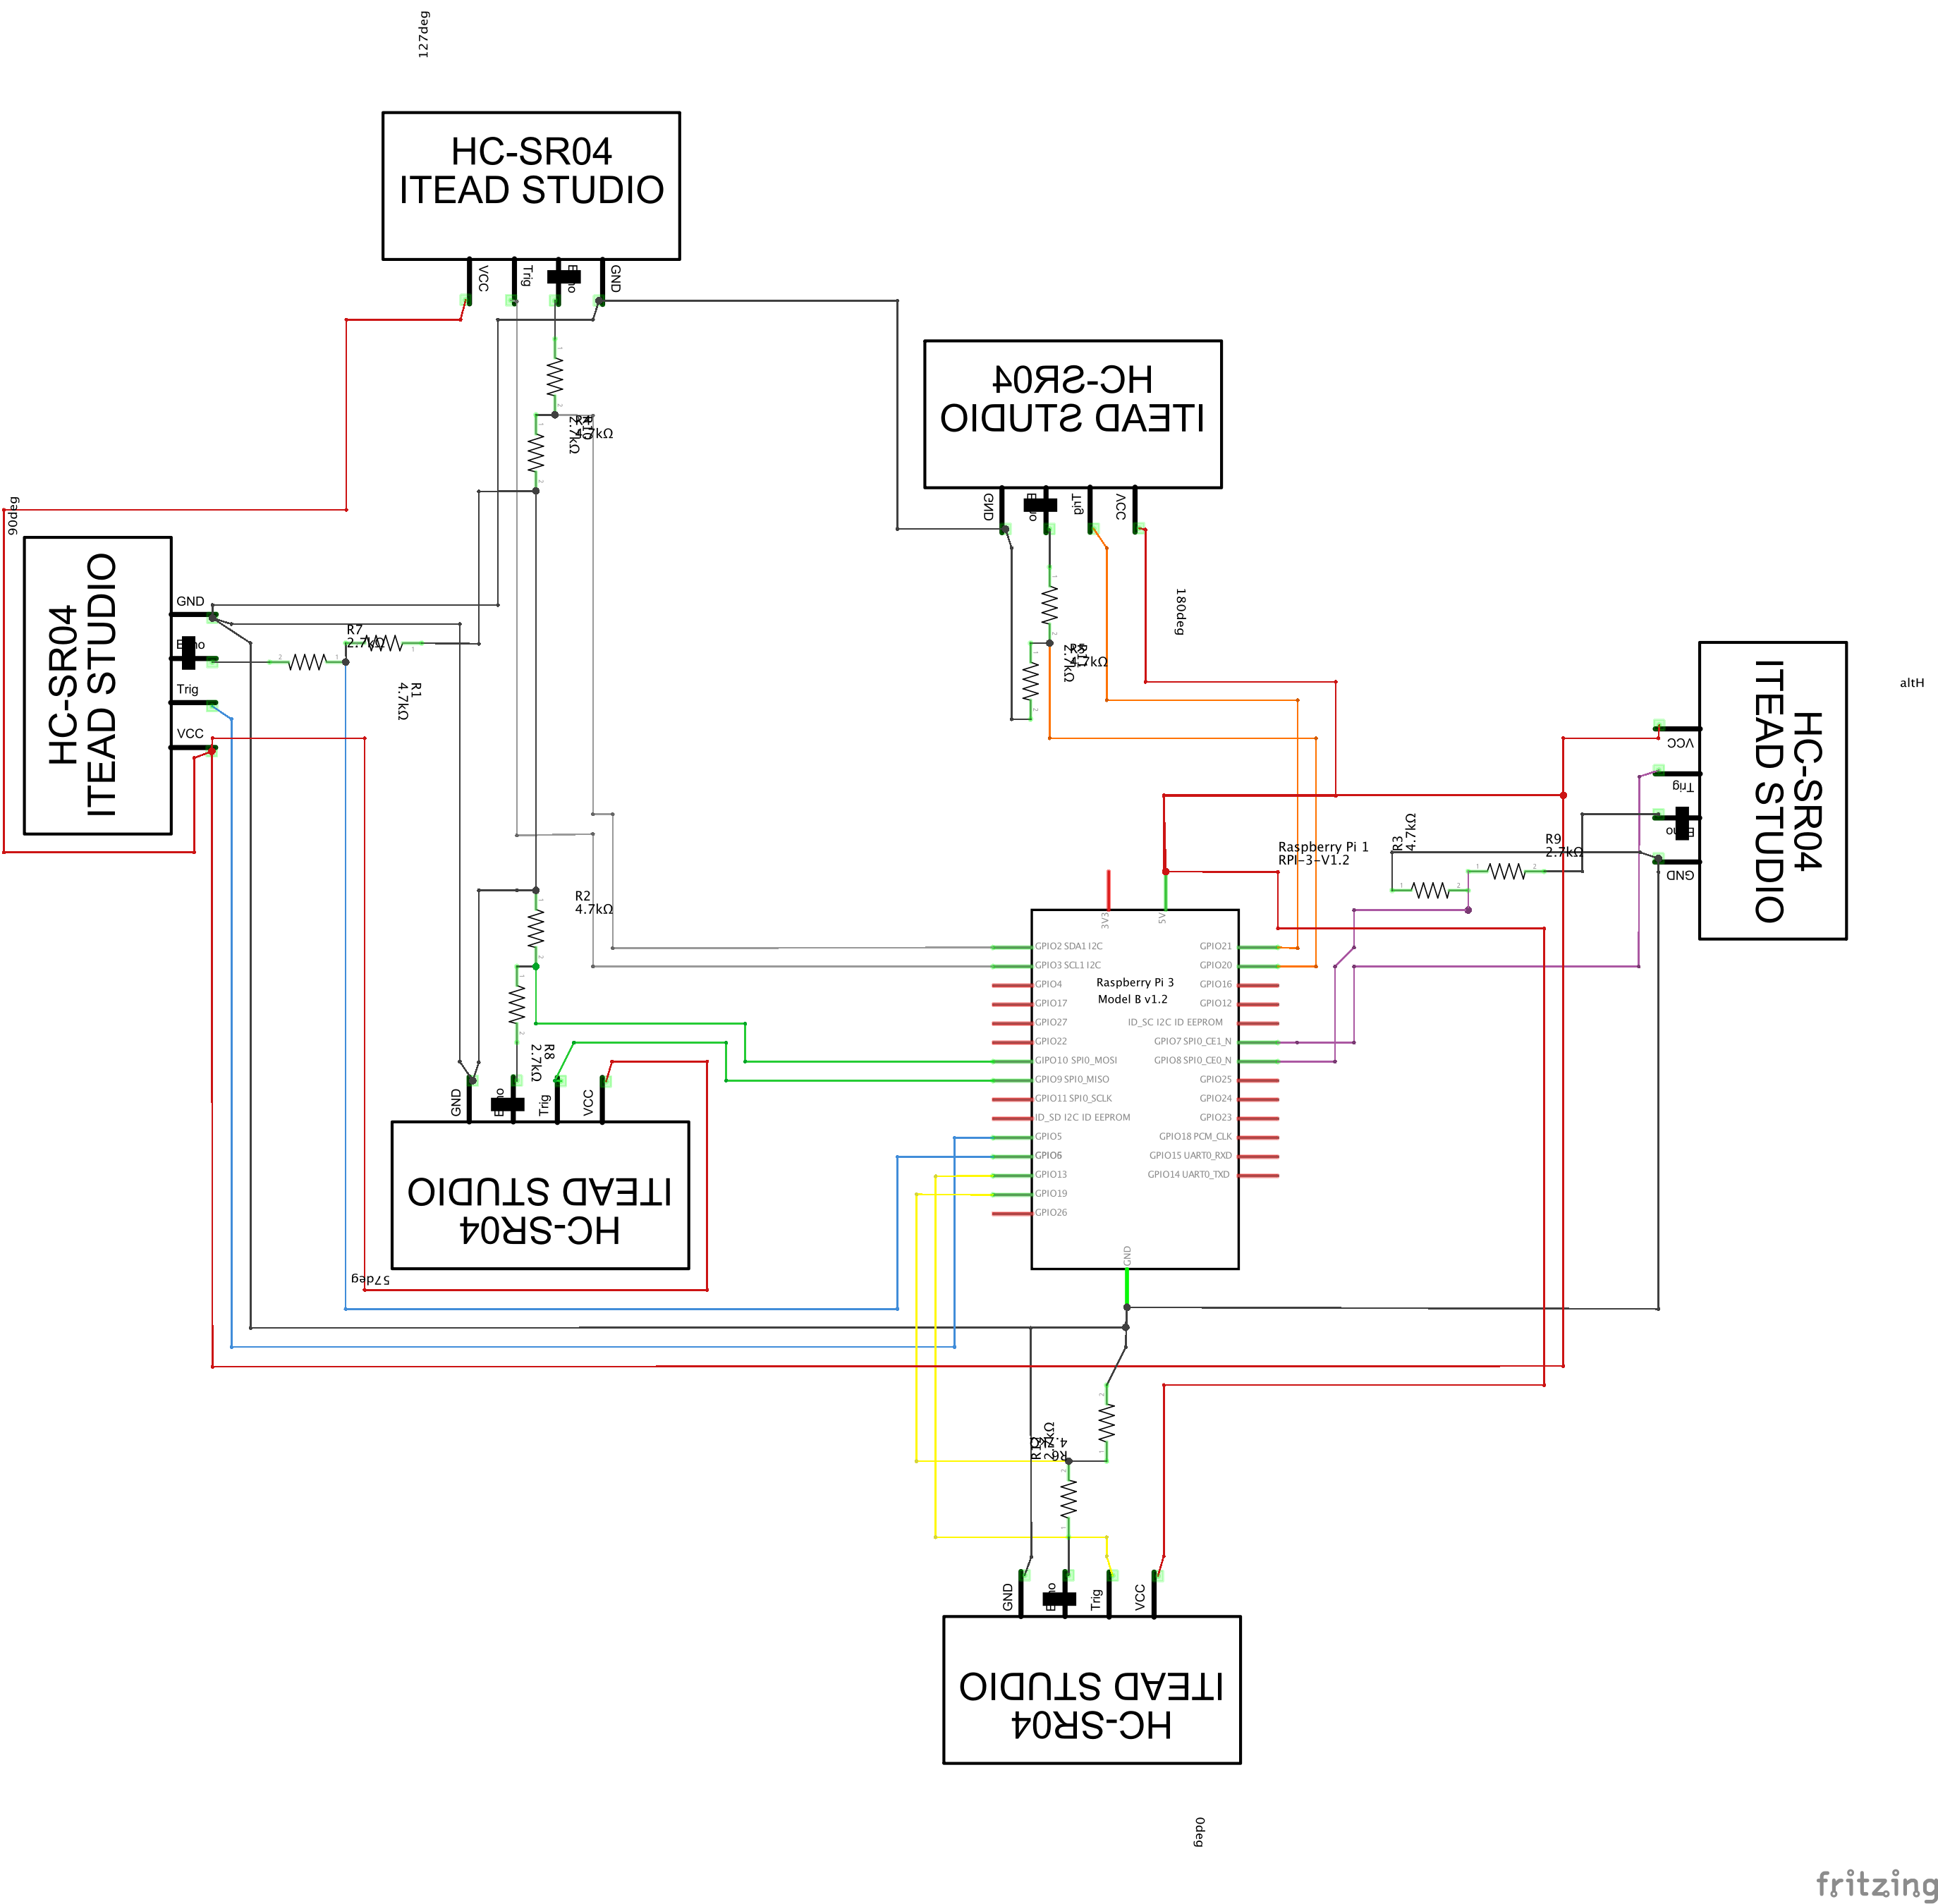
\includegraphics[width=0.7\textwidth]{SR04layout_schem}
	\caption[Diagrama de conexión de sensores a RaspberryPi]{Vista esquemática del conexionado de los sensores a la RaspberryPi.}\label{fig:concepHCPi}
\end{figure}
\item Es importante destacar que el voltaje de salida de los sensores es $5V$, y que por lo tanto puede dañar la RaspberryPi, ya que esta funciona a $3.3V$. Por ello se ha de hacer uso de algún elemento para reducir el voltaje o la corriente suministrada. En la vista esquemática proporcionada, existen divisores de voltaje que permiten reducir este voltaje. 
\item La emisora puede conectarse a un ordenador, y si este la detecta como un \emph{joystick} puede utilizarse para controlar el \emph{drone} a través de la interfaz web. Para ello es necesario configurar la emisora para que proporcione la salida de los canales a través de la conexión USB. 
\end{itemize}


\subsection{Obtención del código fuente}

Para el desarrollo del proyecto se ha utilizado un repositorio Git local, al que se ha establecido un origen remoto en GitHub. Para clonar el proyecto y poder utilizarlo deben seguirse los siguientes pasos:

\begin{enumerate}
\item Abrir un terminal bash. 
\item Moverse hasta el directorio en el que se quiera clonar el repositorio. Para ello puede utilizarse el comando \code{cd}.
\item Clonar el repositorio mediante el comando: \code{git clone git@github.com:mbm0089/GII\_0\_17.02\_SNSI.git} para clonar la rama \emph{master}. Si se desea trabajar en alguna de las ramas en desarrollo, puede usarse el comando \code{git clone -b NOMBRE\_RAMA git@github.com:mbm0089/GII\_0\_17.02\_SNSI.git}
\item Con esto se iniciará la descarga del repositorio completo.
\end{enumerate}

\begin{figure}[H]
	\centering
	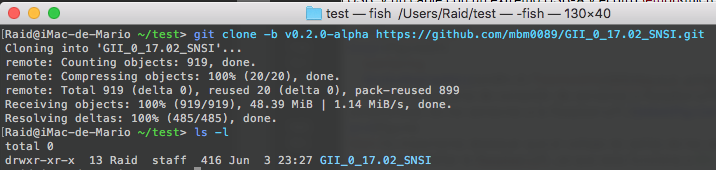
\includegraphics[width=0.9\textwidth]{gitclone}
	\caption[Clonado de repositorio Git]{Clonado del repositorio mediante terminal.}\label{fig:gitclone}
\end{figure}

\section{Compilación, instalación y ejecución del proyecto}
La siguiente sección describirá como instalar las dependencias necesarias, compilar el código y ejecutar el proyecto.

\subsection{Instalación}
\label{subsec:installersh}

El proceso de instalación de dependencias se ha diseñado para que sea totalmente automatizado. 
Bastará con ejecutar el script llamado \emph{installer.sh} de la siguiente manera: 

\begin{enumerate}
\item Abrir una terminal bash.
\item Desplazarse hasta la carpeta del proyecto. Puede usarse el comando \code{cd} para ello.
\item Dar permisos de ejecución al instalador mediante \code{chmod +x installer.sh}.
\item Ejecutar el instalador usando como parámetros el nombre del entorno virtual\footnote{Generalmente, en los proyectos desarrollados en Python, no se instalan las dependencias sobre la instalación base de Python, sino que se usan entornos virtuales. En ellos se crea una copia del intérprete de Python, y se instalan las librerías adicionales sin afectar la instalación del sistema} a crear, y el sistema a instalar (bien el \emph{backend} o el \emph{frontend}, tal que: \code{./installer.sh backendVenv setupBackend.py}, o \code{./installer.sh frontendVenv setupWebUI.py}.
\item Con esto comenzará la instalación de las dependencias necesarias para la ejecución del proyecto. 
\end{enumerate}

Una vez instalado el entorno virtual, este puede configurarse en PyCharm tal y como se explicó en la sección \ref{subsec:pycharm}.


\subsection{Compilación}

La compilación del proyecto es una tarea transparente para el desarrollador. Es el propio intérprete quien se encarga de realizar la compilación de las diferentes clases o scripts en el momento de su ejecución. 

\subsection{Ejecución del proyecto}

Ejecutar el proyecto a través del IDE es un proceso trivial. Una vez establecido los entornos virtuales a utilizar, tanto en local como el entorno remoto para el despliegue del \emph{backend}, bastará con realizar los siguientes pasos: 

\begin{itemize}
\item En el caso de la aplicación web, en la raíz de la carpeta \texttt{/frontend/} se encuentra una clase llamada \emph{droneControlWebUI.py}. Si se ejecuta esta clase, se lanza el servidor web, y se carga la aplicación web creada. Se puede configurar los parámetros del servidor modificando los valores disponibles en la clase de forma muy sencilla.
\begin{figure}[H]
	\centering
	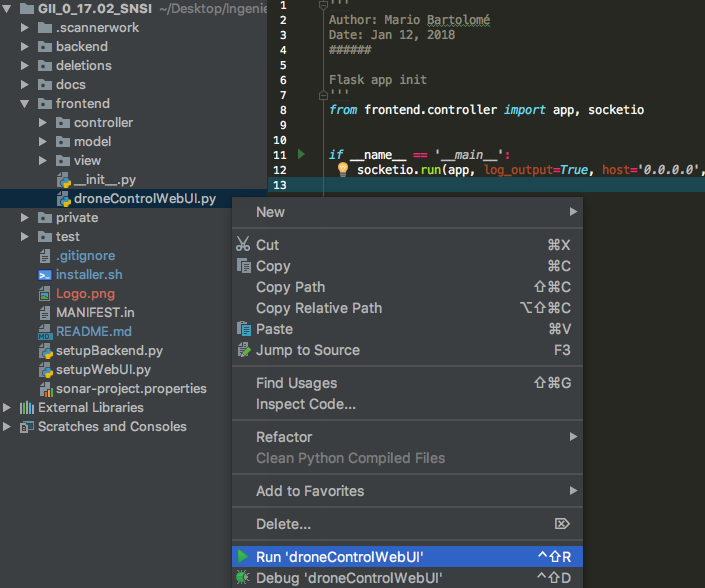
\includegraphics[width=0.9\textwidth]{runwebui}
	\caption[Ejecución de aplicación web]{Ejecución de la aplicación web.}\label{fig:runwebui}
\end{figure}

\item El caso del \emph{backend}, o el código que se ejecuta en la RaspberryPi, es similar. Si se ha seguido el proceso de creación de un intérprete remoto, ver \ref{subsec:pycharm}, éste puede ser seleccionado para ejecutar las clases del proyecto. La clase que debe ejecutarse para lanzar todo el sistema de control del \emph{drone} se encuentra en la carpeta \texttt{/backend/systemControl}, y tiene el nombre de \emph{ctrlWrapper.py}. De esta manera, bastará con establecer la configuración de ejecución de este script para que utilice el intérprete remoto.

\begin{figure}[H]
	\centering
	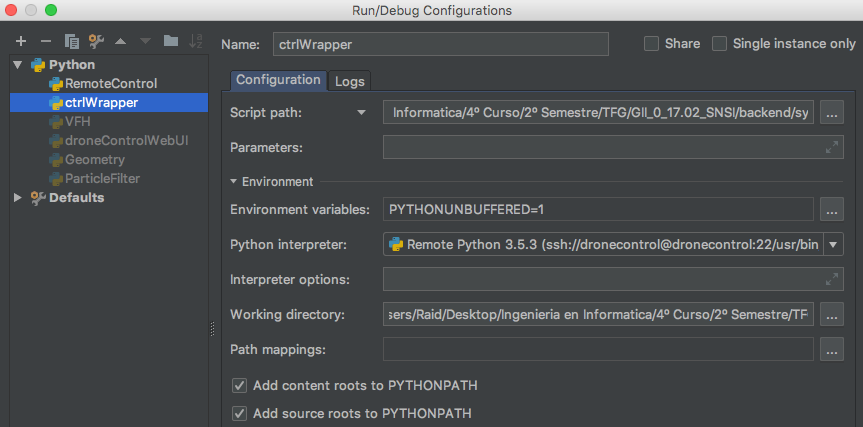
\includegraphics[width=0.9\textwidth]{runbackend}
	\caption[Ejecución del sistema de control]{Ejecución del sistema de control del \emph{drone}.}\label{fig:runbackend}
\end{figure}
\end{itemize}

Si se quisiese ejecutar el proyecto desde una terminal, el proceso requiere de activar el entorno virtual creado, y de establecer una variable de entorno. Bastará con realizar los siguientes pasos:

\begin{enumerate}
\item Abrir un terminal bash.
\item Activar el entorno virtual a utilizar. \code{source EntornoVirtual/bin/activate}.
\item Establecer la variable de entorno \emph{PYTHONPATH} a la raíz del proyecto. Este paso PyCharm lo hace por defecto. \code{export PYTHONPATH=\$(pwd)}.
\item Ejecutar el script deseado desde la raíz del proyecto. \code{python3 -m backend.systemControl.ctrlWrapper} o \code{python3 -m frontend.droneControlWebUI}
\end{enumerate}

\begin{figure}[H]
	\centering
	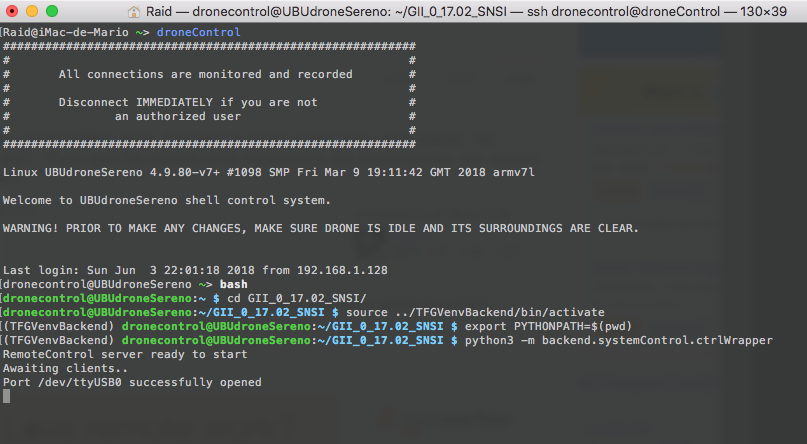
\includegraphics[width=0.9\textwidth]{runconsole}
	\caption[Ejecución del proyecto desde terminal]{Ejecución del proyecto desde un terminal bash.}\label{fig:runconsole}
\end{figure}

\subsection{Añadir nuevos controladores al sistema de control}

Añadir nuevos controladores al sistema de control es relativamente sencillo. Para ello se deben seguir los siguientes pasos, teniendo en cuenta el flujo de trabajo de Git. Cabe destacar que durante la realización de este proyecto, y con la intención de simplificar el flujo de trabajo, dado que solo existe un desarrollador, el flujo de trabajo se ha simplificado creando únicamente ramas para las \emph{release} generadas: 
\begin{enumerate}
\item Crear una nueva rama (\emph{feature branch}) desde la rama de la \emph{release} en la que se está trabajando:\\ \code{git checkout -b new-controller RAMA\_ACTUAL}
  
\item Crear una clase para el \emph{controller} a generar: \texttt{improvedSpeedController.py}, por ejemplo, que implemente los métodos necesarios. Hacer \emph{commit} del nuevo fichero y la lógica generada.
\item Refactorizar el código para mejorar su calidad. Hacer \emph{commit}.
\item Incluir el nuevo controlador generado en el \texttt{ctrlWrapper.py}. Para ello solo se deben proporcionar los métodos requeridos por el controlador principal. 
\item Una vez que se ha implementado correctamente el nuevo controlador, se debe sincronizar en la rama del nuevo desarrollador, anteriormente creada, mediante \code{git push}, y seguidamente incorporar esta rama a la rama de la \emph{release} en desarrollo, y existente en GitHub. Para ello, lo ideal es generar una \emph{pull-request} estableciendo la necesidad de una revisión, pero como se ha comentado solo existe un desarrollador, de manera que en el desarrollo se ha simplificado este paso:\\ \code{git request-pull nombre1erCommit origin\footnote{El origen del proyecto se habrá establecido a https://github.com/mbm0089/GII\_0\_17.02\_SNSI/} new-controller}
\end{enumerate}

De esta forma se generará una \emph{pull-request} en el repositorio remoto hospedado en GitHub. 

Sin embargo, y por comodidad, se ha hecho uso de un cliente de escritorio, que facilita enormemente el flujo de trabajo de Git, de forma que crear una \emph{pull-request} de un \emph{commit} concreto es tan sencillo como dar click derecho sobre el \emph{commit} deseado y pulsar sobre \emph{start a pull-request to origin/ from origin/v0.2.0}, tal y como se muestra en la Figura \ref{fig:pullrequest}.
\begin{figure}[H]
	\centering
	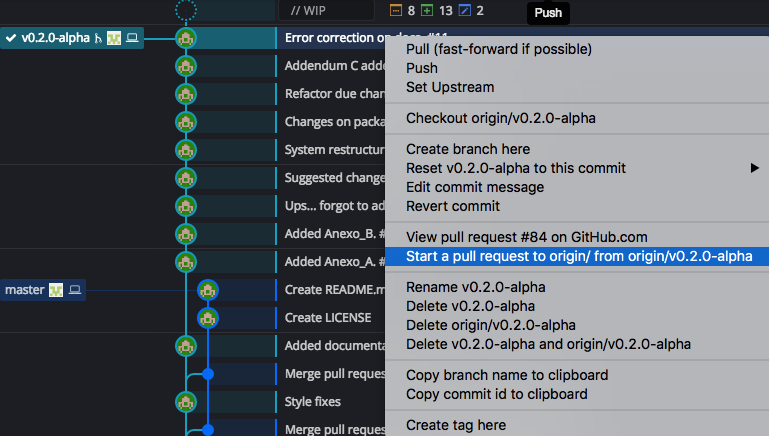
\includegraphics[width=0.9\textwidth]{pullrequest}
	\caption[Creación de \emph{pull-request} desde GitKraken]{Creación de una \emph{pull-request} desde el cliente de escritorio GitKraken.}\label{fig:pullrequest}
\end{figure}
\subsubsection{Programación funcional \emph{VS} Interfaces y diseño por contrato}
Se hace notar que la clase \texttt{ctrlWrapper}, encargada del control de todo el sistema, podría haber definido una metaclase, o interfaz, que los controladores a crear pudiesen implementar. Sin embargo, en aras de la programación funcional, y para explotar la flexibilidad de Python, se ha dejado a la discreción del desarrollador el nombrado, firma, e implementación de las diferentes funciones. 

De esta manera, añadir un nuevo controlador a la lista de controladores priorizados que genera el \emph{ctrlWrapper}, requiere pasar como parámetro las funciones requeridas. 

\subsection{Servicios de integración continua}

Para llevar a cabo una toma de medidas del código generado, se ha hecho uso de una suscripción a \emph{SonarCloud}. Se trata de un servicio proporcionado por \emph{SonarCloud}, de forma que no es necesario instalar un servidor local, sino que se realiza el escaneo del proyecto y los resultados se envían al servicio en línea de \emph{SonarCloud}. 

El escáner a utilizar, se puede descargar de \citep{wiki:getSonarScanner}.

Para ello, se deben seguir los siguientes pasos: 
\begin{enumerate}
\item Abrir un terminal bash.
\item Desplazarse hasta la carpeta del proyecto. Puede usarse el comando \code{cd} para ello.
\item Generar un fichero de configuración de los parámetros requeridos por el escáner de \emph{SonarCloud}, haciendo uso del editor preferido, tal y como puede verse en la Figura \ref{fig:sonarcloudconfig}.
\begin{figure}[H]
	\centering
	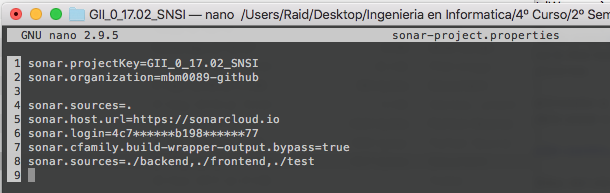
\includegraphics[width=0.9\textwidth]{sonarcloudconfig}
	\caption[Configuración de SonarCloud]{Creación de un fichero de configuración para el servicio online de \emph{SonarCloud}.}\label{fig:sonarcloudconfig}
\end{figure}

Se deberá establecer la clave del proyecto, mediante el atributo \texttt{projectKey}.
Se deberá establecer la organización del proyecto, mediante el atributo \texttt{organization}.
Se deberá establecer la ubicación de las fuentes a utilizar, mediante el atributo \texttt{sources}
Se deberá establecer el host al que conectarse (el escáner es de \emph{SonarQube}, así que pueden enviarse sus resultados a una instancia de un servidor \emph{SonarQube} local), mediante el atributo \texttt{host.url}.
Se deberá establecer un \emph{token} para el login, el cual es generado en la creación del proyecto en \emph{SonarCloud}, mediante el atributo \texttt{login}.
Por último se establecerán los directorios a tener en cuenta, mediante el atributo \texttt{sources}.

\item Ejecutar el escáner de \emph{SonarQube} tal que:\\ \code{sonar-scanner -Dproject.settings=./sonar-project.properties}\footnote{Para ello es necesario que sonar-scanner se encuentre en el \emph{PATH} de ejecución}
\end{enumerate}

Seguidamente, entrando en \href{https://sonarcloud.io/dashboard?id=GII_0_17.02_SNSI}{SonarCloud}, pueden verse los resultados del último análisis, tal y como se muestra en la Figura \ref{fig:sonarcloudresults}
\begin{figure}[H]
	\centering
	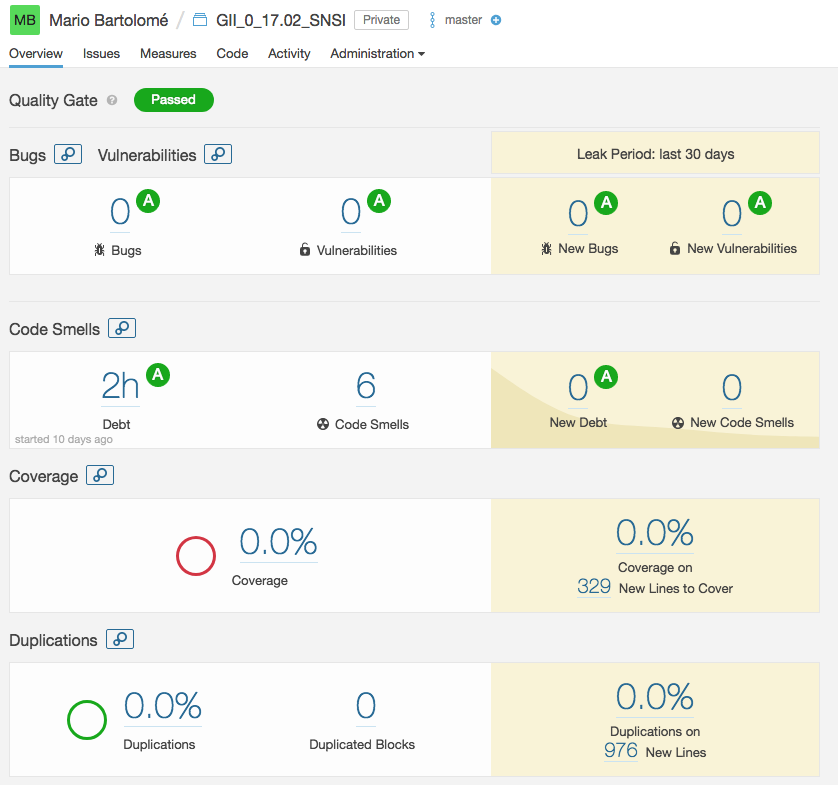
\includegraphics[width=0.9\textwidth]{sonarcloudresults}
	\caption[Resultados de SonarCloud]{Resultados del escaneo del proyecto en \emph{SonarCloud}.}\label{fig:sonarcloudresults}
\end{figure}


\section{Pruebas del sistema}



























